% 本文件是示例论文的一部分
% 论文的主文件位于上级目录的 `main.tex`
\chapter{利用特征选择方法分析粮食生产影响因素}
\label{chapter:3}
本章主要介绍粮食生产模型的第一部分—特征选择,通过分别利用不同特征选择方法对数据集进行处理,以便得到不同算法下的约简数据集与重要特征,并比较不同算法的耗时。
\section{特征选择方法}
影响作物产量的因素会有很多,不同因素对作物的产量会有不同的影响,在生产中如果能抓住其中关键的可控因素,那么便可以在可控范围内尽可能提高作物产量。一般来说,在预测作物产量的过程中,模型中包含的特征越多,其便能包含足够的信息提高预测精度。然而特征数量的增加与预测精度的提高之间的关系并不是线性的,盲目增加特征反而可能会增加模型的复杂度,进而造成过拟合,更多的特征可能会引起更多的噪声,甚至可能降低整体模型的精度。

因此,对于特征过多的数据集,对数据进行属性约简便显得尤为重要,利用特征选择方法将数据集中的关键特征保留下来,删去不重要或高度重叠的特征,仅留下对观测变量较大影响的因素,可以达到在不丢失重要数据信息的前提下约简数据集并保留重要特征的目的。

本节介绍三种不同特征选择方法的理论知识与实验流程,以便得出属性约简结果。
\subsection{基于属性重要度的模糊粗糙集属性约简算法}
\label{chapter:基于属性重要度的模糊粗糙集属性约简算法}
对于本文的核心算法,本文以\cite{基于粗糙集和模糊粗糙集的属性约简研究}中提出的基于属性重要度的模糊粗糙集属性约简算法为启发,选择模糊依赖度作为属性重要度。首先利用聚类算法计算模糊等价类的数量,然后构造模糊隶属函数对连续属性进行模糊化,再利用模糊依赖度计算属性的重要度,然后按照属性重要度对属性进行排序,最后留下重要性排名前10的属性作为约简数据集。

在本实验中,由于实验目标仅为得到各个属性的重要度排名,因而在得到属性的模糊依赖度后没有对属性进行约简以便选出最简属性集,直接选取属性重要度排在前10的特征即可作为算法输出结果。

对于模糊等价类个数的确定,采用模糊$C$均值聚类分别对每个省份的数据进行聚类分析,分别得到不同省份的聚类数,为了统一模糊等价类个数,对19各省份的模糊聚类数求平均得到了平均聚类数为2.8421052631578947,因而选择模糊等价类个数为3类。

在确定模糊等价类个数后,就要确定模糊隶属函数了。由于模糊隶属函数的确定需要根据数据分布及特点确定,故实验中对各个属性绘制了箱线图,分别观察其分布特点,发现大部分数据集中在某一个区间内,仅有少部分数据较为分散,因此选择最常用的梯形隶属函数作为模糊隶属函数。然后根据箱线图中显示的25分位线、中位线及75分位线,对各个省份属性分位线进行求平均值,得到数据的平均分布,再根据数据分布特点确定梯形隶属函数的四个决定点分别为0.23、0.37、0.43及0.57。由此构造出三个模糊等价类的模糊隶属函数如\ref{fig:membership_foodsecurity}。

\begin{figure}[htbp]
      \centering
      \resizebox{\textwidth}{!}
      {
      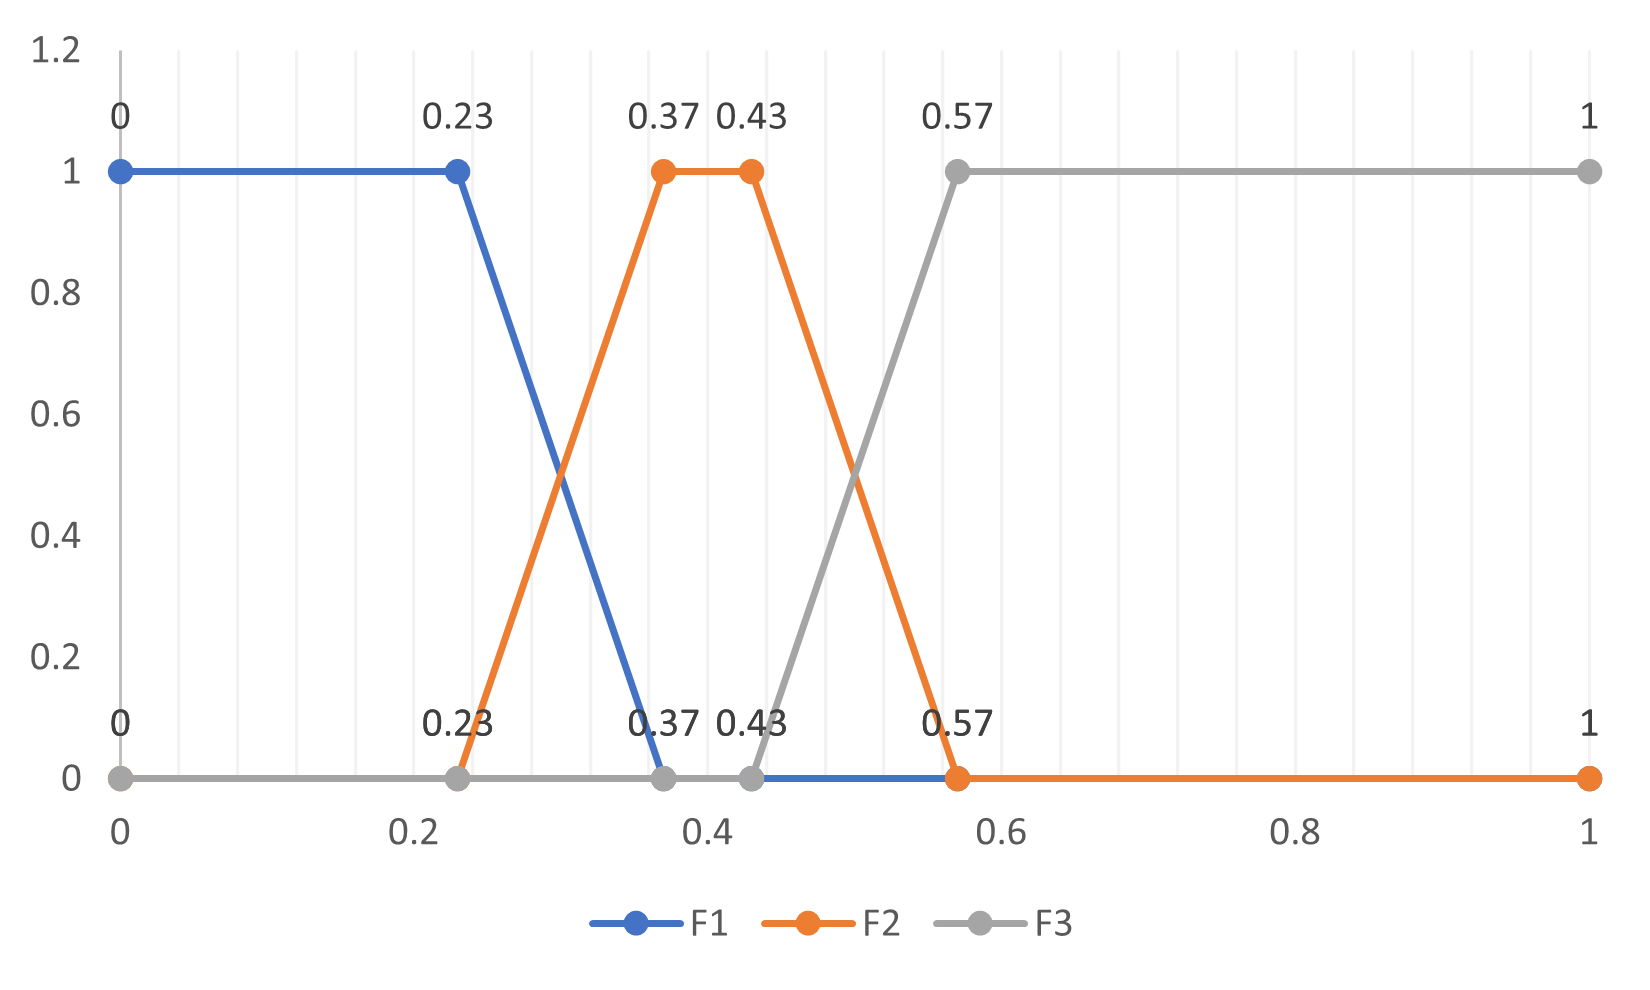
\includegraphics{figs/membership_foodsecurity.png}
      }
      \caption{玉米生产数据模糊隶属函数}
      \label{fig:membership_foodsecurity}
\end{figure}

在确定模糊隶属函数后,按照\ref{chapter:0105}所述的\nameref{alg:FRARAlgorithm}流程,首先构造模糊环境将不同量纲数据归一化到[0,1]区间(在\nameref{subsection:DataCleaning}部分已完成),然后利用\ref{fig:membership_foodsecurity}中的模糊隶属函数将玉米生产数据模糊化,得到三个模糊等价类,然后利用\nameref{def:模糊正域隶属度}计算每个对象对任一条件属性的模糊隶属度,进而由定义\ref{def:模糊依赖度}得到每个条件属性对决策属性的模糊依赖度,最后取该属性的模糊依赖度为其属性重要度,进而得到了每个属性的重要性排名,进而得到该方法下最重要的10个属性。

基于属性重要度的模糊粗糙集属性约简算法作为本文的核心方法,其原理与算法已在\ref{chapter:0105}进行了详尽的阐述。在特征选择过程中以每个省份的粮食生产数据作为一个研究单元,将26个解释变量作为条件属性集,将每亩玉米产量作为决策属性,采用模糊粗糙集属性约简算法进行属性约简,得到每个属性的重要度,计算属性约简耗时,并将每个条件属性的属性重要度作为每个解释变量对玉米产量的影响程度,并按照其属性重要度对属性进行排序,只保留重要性前10的变量作为约简数据集。

% 粗糙集属性约简算法是一种特征选择算法,其基于粗糙集理论,通过删除冗余和不相关的属性,得到一个最小的特征子集,使得该子集可以准确地刻画数据集中的规律和特征,进而达到约简数据集与特征选择的目的。属性约简的目的就是在保证分类准确率的前提下,去除一些无关的条件属性,以减少模型的复杂度和提高模型的泛化能力。\cite{2008Attributes}

% 粗糙集属性约简算法的优点在于具有较好的鲁棒性,能够处理包含不确定性和噪声的数据集,但缺点在于计算复杂度高,且传统的粗糙集属性约简算法只能处理二元属性,无法处理连续属性和模糊属性等不确定性问题。\cite{2020Regional}

% 而基于粗糙集方法的模糊粗糙集属性约简算法作为粗糙集属性约简算法的改进,融合了模糊集合理论和粗糙集理论,能够处理不确定性问题,包括模糊属性和连续属性等,更高的准确性、可靠性及更广泛的应用场景,不仅局限于粗糙集属性约简算法的预测与回归问题。\cite{模糊粗糙集理论研究进展}因在本文实验中需要计算出每个特征的重要性,因此选择基于属性重要度的模糊粗糙集属性约简算法作为研究算法。


\subsection{基于Lasso的特征选择算法}

Lasso(Least Absolute Shrinkage and Selection Operator)是一种线性回归的正则化方法,它在多元线性回归模型的基础上,通过在损失函数中添加$L_1$正则化项来实现特征选择。因添加了$L_1$正则化项的原因,其可以将一些系数收缩为零,从而使得一些系数为零的特征对预测结果没有贡献,进而达到特征选择的效果。下面将从多元线性回归模型开始介绍Lasso的原理。

\subsubsection{多元线性回归模型}
多元线性回归模型是一种用于建模和预测的统计模型,它建立了自变量(特征)和因变量之间的线性关系。假设有一个目标变量(因变量)$Y$和一组自变量(特征)$X_1, X_2,\cdots, X_p$,多元线性回归模型可以表示为:
$$Y=\beta_{0}+\beta_{1} X_{1}+\beta_{2} X_{2}+\ldots+\beta_{p} X_{p}+\varepsilon.$$
其中,$Y$是目标变量的观测值,$\beta_{0}, \beta_{1}, \beta_{2}, \ldots, \beta_{p}$  是模型的系数,表示自变 量对目标变量的影响,$\varepsilon$是误差项,表示模型无法解释的随机误差。

模型的目标是找到最优的系数  $\beta_{0}, \beta_{1}, \beta_{2}, \ldots, \beta_{p} $,使得模型的预测值与实际观测值之间的残差(误差的平方和)最小化。这通常通过最小二乘法来实现,即最小化残差平方和。

然而,多元线性回归模型存在一个问题,即在面对高维数据或特征共线性时,模型的性能可能下降或不稳定。在这种情况下,正则化方法可以用于改善模型的性能和稳定性。Lasso(Least Absolute Shrinkage and Selection Operator)和岭回归(Ridge Regression)都是常见的正则化方法\cite{基于Lasso的我国股票价格影响因素分析}。

\subsubsection{岭回归}

岭回归是多元线性回归的一种扩展方法,通过引入L2正则化项来控制模型的复杂度。L2正则化项是模型系数的平方和乘以一个正则化参数(α),用于惩罚模型系数的大小。岭回归的目标是通过最小化残差平方和和L2正则化项,获得一个系数较小的模型。岭回归的目标函数可以表示为:
$$\min _{\beta_{0}, \beta} \frac{1}{2 n} \sum_{i=1}^{n}\left(y_{i}-\beta_{0}-\sum_{j=1}^{p} x_{i j} \beta_{j}\right)^{2}+\alpha \sum_{j=1}^{p}(\beta_{j})^2.$$
岭回归的$L_2$正则化项对模型系数进行约束,使得模型系数的取值相对较小,从而减小过拟合的风险。与多元线性回归相比,岭回归倾向于得到一个稳定且较简单的模型,而不会将系数完全缩小为零\cite{基于Lasso的我国股票价格影响因素分析}。

\subsubsection{Lasso}
Lasso和岭回归的区别主要在于正则化项的不同。岭回归使用$L_2$正则化,对所有特征进行缩小,适用于具有多个相关特征的问题;Lasso使用$L_1$正则化,可以实现特征选择和稀疏性,适用于具有少量重要特征的问题。Lasso的目标函数为:
$$L(\beta)=\sum_{i=1}^{n}\left(y_{i}-\beta_{0}-\sum_{j=1}^{p} x_{i j} \beta_{j}\right)^{2}+\lambda \sum_{j=1}^{p}\left|\beta_{j}\right|.$$
其中,$n$是样本数,$p$是特征数,$\beta$ 是 $p$ 维系数向量,$\beta_0$ 是截距,$x_{ij}$ 是第 $i$ 个样本第 $j$ 个特征的取值,$y_i$ 是第 $i$ 个样本的目标变量取值,$\lambda$ 是正则化系数。

在存在共线性时,Lasso可能选择其中一个相关特征,而岭回归会将系数平均分配给相关特征。因此Lasso方法的优点在于能够自动选择对目标变量有显著影响的特征,并将其他不重要的特征的系数缩小为零,从而实现特征选择和模型简化。

在Lasso回归中,优化的目标是在保证拟合精度的同时,尽可能使得特征系数之和最小。而正则化系数$\lambda$控制着特征选择的程度,当 $\lambda$ 较大时,意味着正则化罚项的在目标函数中的权重较大,目标函数在优化过程中会因正则化项惩罚较大而使得大部分系数被压缩至零,只有少量的系数会保留,从而实现特征选择的效果\cite{基于Lasso的我国股票价格影响因素分析}。

在Lasso算法实现中,对于Lasso的正则化参数分别选择$\alpha=[0.001, 0.01, 0.1, 1, 10]$,最大迭代次数为1000000。并选用五折交叉验证对模型进行拟合,并计算模型拟合的耗时,选出最佳的模型估计器,并得到其最佳线性系数,那么不同特征对应的系数就是该特征在Lasso模型中的重要度。最后按照最佳线性系数对特征进行排序,并选取前10位特征作为约简数据集。

\subsection{基于随机森林变量重要性的特征选择算法}
随机森林是一种集成学习方法,它由多个决策树组成。每个决策树都是基于不同的随机样本和随机特征训练得到的。在随机森林训练过程中,每个特征都会被分配一个重要性分数,这个分数衡量了该特征对模型预测性能的贡献程度。而特征重要性分数一般有两种计算方法:信息增益和基尼系数。信息增益使用熵和条件熵来计算特征对模型的贡献,基尼系数通过计算特征在样本中出现的概率分布来评估其对模型的影响。在这两种方法中,特征重要性分数越高说明该特征对模型的贡献越大。

基于随机森林变量重要性的特征选择算法通过计算每个特征在随机森林中的重要性分数,按照特征重要性分数从大到小的顺序,逐步选择特征,直到达到预先设定的特征数或特征重要性分数的阈值为止,最终得到的特征集包含对预测结果最有影响的特征。这种方法相对于其他特征选择方法的优点在于其可以同时考虑多个特征之间的互相影响,避免了因单独分析某个特征而忽略了全局其余特征的问题。同时模型具有较好的鲁棒性和泛化能力,可以有效避免模型过拟合问题。
\subsubsection{随机森林模型原理}

随机采样:随机森林的第一步是从原始训练数据集中进行随机采样,构建多个训练子集。采样是有放回地进行的,意味着同一个样本可以在多个子集中出现。通过随机采样,每个训练子集都会略有差异,使得每个子集都具有随机性。这种随机性能够减小模型对训练数据集中的噪声和过拟合的敏感度。

随机特征选择:在随机森林的每个决策树节点进行分裂时,不是使用所有特征,而是随机选择一个特征子集。这样可以减少特征间的相关性,增加模型的多样性。常用的特征选择方法是随机选择$m$个特征,其中$m$是总特征数的平方根或者对数值(取整数部分)。随机特征选择使得每个决策树都只考虑部分特征,增加了模型的多样性。

决策树的构建:对于每个子集和每棵决策树,使用常规的决策树算法(如ID3、CART等)来构建决策树模型。决策树的构建过程中,通过节点的分裂,将样本划分为不同的类别或者进行回归预测。节点的分裂依据是特征的选择,该选择在随机特征选择阶段已经确定。决策树的构建过程会递归进行,直到达到停止条件(如达到最大深度、节点中的样本数小于阈值等)。

预测与集成:在随机森林中,回归问题的预测结果是所有决策树的预测值的平均值。而对于分类问题,采用投票的方式,选择预测结果最多的类别作为最终预测结果。这种集成方式能够平衡不同决策树的预测结果,提高了模型的鲁棒性和准确性。预测与集成过程是随机森林模型的最后一步,通过汇总多个决策树的预测结果来获得最终的预测值或分类结果\cite{随机森林算法优化研究}。
\subsubsection{随机森林变量重要性计算方法}

随机森林通过测量变量在模型中的使用频率和节点分裂时的效果来评估变量的重要性。常用的计算方法有信息增益和基尼系数。

信息增益:随机森林中的每个决策树都可以计算节点分裂时的信息增益,衡量了该特征对于样本分类的贡献程度。通过计算每个特征在所有决策树中的平均信息增益,得到变量的重要性。信息增益越大,说明该特征在随机森林中的重要性越高。

基尼系数:基尼系数是另一种衡量节点分裂的指标,表示了样本被错误分类的概率。计算方式类似于信息增益,通过计算每个特征在所有决策树中的平均基尼系数来评估变量的重要性。基尼系数越小,说明该特征在随机森林中的重要性越高。

通过计算每个特征在所有决策树中的平均信息增益或基尼系数,可以得到变量重要性的排序。较高的变量重要性意味着该特征对模型的预测性能具有更大的贡献\cite{随机森林算法优化研究}。

在随机森林变量重要性算法实现上,设置决策数数量为100,随机种子为42,采用随机森林回归器对玉米生产数据进行训练,得到最佳的随机森林模型,并采用基尼系数计算最佳模型的变量重要性,并按照变量重要性对特征进行排序,得到重要性前10的特征作为约简属性。

\section{对粮食生产数据进行属性约简}
\begin{figure}[htbp]
      \centering
      \resizebox{\textwidth}{!}
      {
      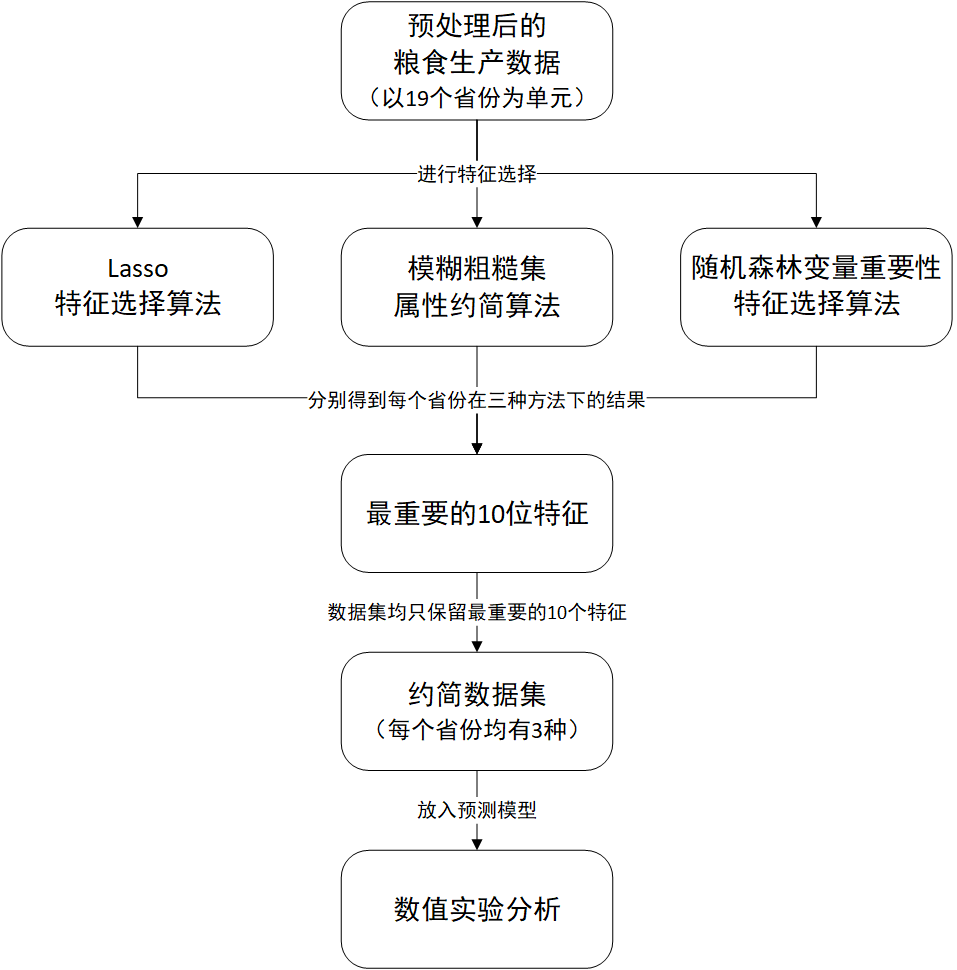
\includegraphics{FeatureSelection}
      }
      \caption{特征选择流程图}
      \label{fig:FeatureSelectionTime}
    \end{figure}
    在特征选择中,分别选择模糊粗糙集属性约简算法(Fuzzy Rough Set Attribute Reduction,以下简记FRAR)、Lasso特征选择算法(Least Absolute Shrinkage and Selection Operator,以下简记Lasso)、随机森林变量重要性特征选择算法(Random Forest,以下简记RF)作为特征选择研究方法,以全国19个省份中每个省份2004-2021年共计26个特征数据为研究对象分别进行特征选择,分别选出每个省份在三种不同方法下最重要的10个特征,并分别计算不同方法的算法耗时。然后对数据集进行属性约简,约简数据集仅保留不同方法下最重要的10位特征,其中每个省份有三份数据集,分别为三种特征选择方法下的约简数据集,之后再对数据集进行数值实验。整体流程图见\ref{fig:FeatureSelectionTime}。
% \begin{algorithm}[htbp]
%       \caption{特征选择算法} %算法的名字
%       \label{alg:FeatureSelectionAlgorithm}
%       \hspace*{0.02in} {\bf 输入:} %算法的输入, \hspace*{0.02in}用来控制位置,同时利用 \\ 进行换行
%       各个省份预处理后的数据AllData\\
%       \hspace*{0.02in} {\bf 输出:} %算法的结果输出
%       各个省份约简后的数据集ReducedData, 特征选择结果ReducedFeatures, 特征选择耗时RunningTime
%       \begin{algorithmic}
%       \For{循环每个省份的数据Data} % For 语句,需要和EndFor对应
%           \State 将Data拆分为特征矩阵X与被解释变量y
%           \State 分别用三种方法进行特征选择
%             \If{FRAR} % If 语句,需要和EndIf对应
%                 \State 计算程序耗时
%                 \State 创建迭代特征的索引     
%                 \State 计算任意两个属性之间的依赖度dep
%                 \State 计算每个属性的不确定度ind
%                 \State 计算每个属性的相对重要度importance=dep-ind
%                 \State 对所有属性按照相对重要度进行排序
%             \ElsIf{Lasso}
%                 \State 选择正则化参数$\alpha$为0.001,0.01,0.1,1,10
%                 \State 最大迭代次数为1000000
%                 \State 交叉验证策略设置为cv=5
%                 \State 计算程序耗时
%                 \State 采用5折交叉验证对Lasso模型进行拟合
%                 \State 选出最佳模型的估计器BestModel与其最佳线性系数coefs
%                 \State 按照最佳线性系数对特征进行排序
%             \ElsIf{RF}
%                 \State 创建随机森林回归器RandomForestRegressor
%                 \State 决策树数量nEstimators设置为100,随机种子为42
%                 \State 计算程序耗时
%                 \State 用随机森林回归器进行训练
%                 \State 提取最佳随机森林模型的特征重要性
%                 \State 按照特征重要性进行排序
%             \EndIf
%           \State 选出排在前10的特征得到特征选择结果ReducedFeatures
%           \State 将原数据集删去未排在重要性前10的特征得到约简数据集ReducedData
%           \State 得到每个省份不同特征选择方法的特征选择耗时RunningTime
%       \EndFor\\
%       \Return 每个省份的约简数据集、特征选择结果及特征选择耗时
%       \end{algorithmic}
%       \end{algorithm}

% 其中,三种特征选择方法进行特征选择的算法实现过程见\nameref{alg:FeatureSelectionAlgorithm},在这里用一层循环实现,循环遍历每个省份的数据,输入数据为excel表格,其中每个sheet存放由\ref{subsection:DataCleaning}进行预处理后的一个省份自2004-2021年的26个解释变量数据。

% 在特征选择方法的算法流程中,模型选择了最常用的参数。对于粗糙集方法选择了基于属性重要度的模糊粗糙集属性约简算法,利用列表推导式分别算出任意两个属性之间的依赖度与每个属性的不确定度,再将依赖度减去不确定度计算出每个属性的相对重要度,最后根据相对重要度对属性进行排序。对于Lasso方法,正则化参数$\alpha$为0.001、0.01、0.1、1、10,最大迭代次数设置为1000000,并采用5折交叉验证进行拟合,得到最佳模型,并导出最佳模型中每个特征的线性系数,再根据线性系数进行排序。对于随机森林模型,决策树数量设置为100,随机种子设置为42,创建随机森林回归器并训练得到最佳模型,提取出最佳模型的特征重要性,再按照特征重要性进行排序。最后得到每个省份在不同特征选择方法下的特征选择结果、特征选择耗时与约简数据集。
\section{特征选择结果}
本节将展示对三种不同特征选择方法的特征选择结果,包括特征选择后的特征与算法耗时,约简数据集将在\ref{chapter:3}中进行数值实验。
\subsection{属性约简后的结果}
每个省份的数据集经过特征选择后,分别得到了不同方法下最重要的10个特征,结果见\ref{table:Feature5_FRAR}(在此仅展示FRAR的前5位特征,其余见附录),并据此数据集进行属性约简,得到各省份在不同方法下的约简数据集,以便后续进行数值实验分析。
\begin{table}[htbp]
      \centering
      \caption{FRAR:各省份前5位特征}
      \label{table:Feature5_FRAR}
      \resizebox{\textwidth}{!}
      {
      \csvautobooktabular{data/ReducedFeatures_FRAR.csv}
      }
\end{table}

\subsection{算法耗时比较}

% 将csv文件载入数据库
\DTLloaddb{RunningTime}{data/RunningTime.csv}
\begin{table}[htbp]
      \centering
      \caption{特征选择算法耗时比较(单位:秒)}
      \label{table:RunningTime}
      \csvautobooktabular{data/RunningTime.csv}
\end{table}

在特征选择过程中,分别计算了各省份在不同算法下的特征选择耗时,其中对三种方法的计时标准进行了统一,计时部分均只有三种特征选择方法的函数调用主体,三个函数输入均为各省的玉米生产数据,输出均为所有变量的重要性,通过统一函数的输入与输出来比较不同算法的耗时。结果如\ref{table:RunningTime}所示。可以看到,Lasso平均耗时大致为随机森林变量重要性方法RF平均耗时的两到三倍,模糊粗糙集属性约简算法FRAR的平均耗时为Lasso的一半,为RF的1.5倍,FRAR方法的耗时较Lasso快,稍慢于RF。

这也说明了模糊粗糙集属性约简算法相较于基于回归方法的Lasso不需要大量的交叉验证进行拟合优化,因而算法效率较Lasso高。而与RF相比,FRAR算法多出的耗时相较于Lasso能够忍受,其耗时大部分花费在对数据进行模糊化过程中的计算模糊隶属度方面,如果能在这方面对代码进行进一步的优化,则其算法效率还可进一步提高。




%%%%%%%%%%%%%%%%%%%%%%%%%%%%%%%%%%%%%%%%%%%%%%%%%%%%%%%%%%%%%%%%%%%%%
% \section{学习资源}

% 对于数学公式的排版在\enquote{lshort-zh-cn.pdf}的第四章给出了基本的使用方法,
% 请大家阅读学习。其内容对大多数人来说已经足够用了,但是如果不能解决问题的话
% 建议大家求助于搜索引擎或者有经验的人,这也不失为一个好办法。

% 常见的几个学习\LaTeX{}数学公式排版的资源链接如下:

% \begin{itemize}
%   \item 数学排版常见问题集:
%         \url{https://www.latexstudio.net/index/details/index/mid/635}
%   \item \pkg{amsmath}手册中译:
%         \url{https://www.latexstudio.net/index/details/index/mid/706}
%   \item \LaTeX{}公式备忘单:
%         \url{https://www.latexstudio.net/index/details/index/mid/1052.html}
% \end{itemize}

% \section{公式排版与注解}

% 按我校学位论文排版要求,公式排版需要行间居中排版,公式编号按照一级标题(章)
% 连续编号(按章)并加小括号,不加导引线。类似这些细节\nwafuthesis{}模板都已进
% 行了设置。在撰写论文中只要将公式置于\env{equation}环境,并用\cs{label}命令
% 添加标签后用\cs{ref}或\cs{eqref}命令引用该公式即可。对于多行公式可以在
% \env{equation}环境中使用\env{aligned}环境实现排版。

% 需要注意的是,公式解释下面的\enquote{式中}两字需要左起顶格编排,后接符号及
% 其解释;解释顺序为先左后右,先上后下;解释与解释之间用中文分号“;”分隔。
% 此时可以用\cs{noindent}命令临时取消首行缩进,在解释完公式符号后,再次正常
% 用空行进行分段便可自动恢复段落首行缩进。

% 例如:勾股定理可以表示为\ref{eq:gougu}

% \begin{equation}
%   a^2+b^2=c^2\label{eq:gougu}
% \end{equation}

% \noindent
% 式中,$a$是一条直角边边长;$b$是另一条直角边边长;$c$是斜边边长。

% 在公式解释结束后,段落缩进应复位至首行缩进2个汉字的模式。

% \section{模板提供的数学环境}

% \nwafuthesis{} 提供了一系列预定义的数学环境,详情见\nwafuthesis{}说明书的表6。
% 其使用样例有以下7种形式。

% \subsection{axiom公理环境}

% \begin{axiom}[欧几里得距离]
% 点$\mathbf{p}$与点$\mathbf{q}$的\textbf{欧几里德距离},是连接两点的线段
% ($\overline{\mathbf{pq}}$)的长度。

% 在笛卡尔坐标系下,如果 $n$维欧几里得空间下的两个点 $\mathbf{p}=(p_1, p_2,
% \dots, p_n)$ 与点$\mathbf{q} = (q_1, q_2, q_3, \dots, q_n)$,那么点$\mathbf{p}$
% 与点$\mathbf{q}$的距离,或者点$\mathbf{q}$与点$\mathbf{p}$的距离,由
% \autoref{equ:1}定义:
% \begin{align}
% d(\mathbf{p},\mathbf{q}) = d(\mathbf{q},\mathbf{p}) & = \sqrt{(q_1-p_1)^2
%                          + (q_2-p_2)^2 + \cdots + (q_n-p_n)^2} \notag \\
% \label{equ:1}
% & = \sqrt{\sum_{i=1}^n (q_i-p_i)^2}
% \end{align}
% \end{axiom}

% \subsection{corollary推论环境}

% \begin{corollary}[欧几里得距离]
% 点$\mathbf{p}$与点$\mathbf{q}$的\textbf{欧几里德距离},是连接两点的线段
% ($\overline{\mathbf{pq}}$)的长度。

% 在笛卡尔坐标系下,如果 $n$维欧几里得空间下的两个点 $\mathbf{p}=(p_1, p_2,
% \dots, p_n)$ 与点$\mathbf{q} = (q_1, q_2, q_3, \dots, q_n)$,那么点$\mathbf{p}$
% 与点$\mathbf{q}$的距离,或者点$\mathbf{q}$与点$\mathbf{p}$的距离,由
% \autoref{equ:2}定义:
% \begin{align}
% d(\mathbf{p},\mathbf{q}) = d(\mathbf{q},\mathbf{p}) & = \sqrt{(q_1-p_1)^2
%                          + (q_2-p_2)^2 + \cdots + (q_n-p_n)^2} \notag \\
% \label{equ:2}
% & = \sqrt{\sum_{i=1}^n (q_i-p_i)^2}
% \end{align}
% \end{corollary}

% \subsection{definition定义环境}

% \begin{definition}[欧几里得距离]
% 点$\mathbf{p}$与点$\mathbf{q}$的\textbf{欧几里德距离},是连接两点的线段
% ($\overline{\mathbf{pq}}$)的长度。

% 在笛卡尔坐标系下,如果 $n$维欧几里得空间下的两个点 $\mathbf{p}=(p_1, p_2,
% \dots, p_n)$ 与点$\mathbf{q} = (q_1, q_2, q_3, \dots, q_n)$,那么点$\mathbf{p}$
% 与点$\mathbf{q}$的距离,或者点$\mathbf{q}$与点$\mathbf{p}$的距离,由
% \autoref{equ:3}定义:
% \begin{align}
% d(\mathbf{p},\mathbf{q}) = d(\mathbf{q},\mathbf{p}) & = \sqrt{(q_1-p_1)^2
%                          + (q_2-p_2)^2 + \cdots + (q_n-p_n)^2} \notag \\
% \label{equ:3}
% & = \sqrt{\sum_{i=1}^n (q_i-p_i)^2}
% \end{align}
% \end{definition}

% \subsection{example示例环境}

% \begin{example}[欧几里得距离]
% 点$\mathbf{p}$与点$\mathbf{q}$的\textbf{欧几里德距离},是连接两点的线段
% ($\overline{\mathbf{pq}}$)的长度。

% 在笛卡尔坐标系下,如果 $n$维欧几里得空间下的两个点 $\mathbf{p}=(p_1, p_2,
% \dots, p_n)$ 与点$\mathbf{q} = (q_1, q_2, q_3, \dots, q_n)$,那么点$\mathbf{p}$
% 与点$\mathbf{q}$的距离,或者点$\mathbf{q}$与点$\mathbf{p}$的距离,由
% \autoref{equ:4}定义:
% \begin{align}
% d(\mathbf{p},\mathbf{q}) = d(\mathbf{q},\mathbf{p}) & = \sqrt{(q_1-p_1)^2
%                          + (q_2-p_2)^2 + \cdots + (q_n-p_n)^2} \notag \\
% \label{equ:4}
% & = \sqrt{\sum_{i=1}^n (q_i-p_i)^2}
% \end{align}
% \end{example}

% \subsection{lemma引理环境}

% \begin{lemma}[欧几里得距离]
% 点$\mathbf{p}$与点$\mathbf{q}$的\textbf{欧几里德距离},是连接两点的线段
% ($\overline{\mathbf{pq}}$)的长度。

% 在笛卡尔坐标系下,如果 $n$维欧几里得空间下的两个点 $\mathbf{p}=(p_1, p_2,
% \dots, p_n)$ 与点$\mathbf{q} = (q_1, q_2, q_3, \dots, q_n)$,那么点$\mathbf{p}$
% 与点$\mathbf{q}$的距离,或者点$\mathbf{q}$与点$\mathbf{p}$的距离,由
% \autoref{equ:5}定义:
% \begin{align}
% d(\mathbf{p},\mathbf{q}) = d(\mathbf{q},\mathbf{p}) & = \sqrt{(q_1-p_1)^2
%                          + (q_2-p_2)^2 + \cdots + (q_n-p_n)^2} \notag \\
% \label{equ:5}
% & = \sqrt{\sum_{i=1}^n (q_i-p_i)^2}
% \end{align}
% \end{lemma}

% \subsection{proof证明环境}

% \begin{proof}[欧几里得距离]
% 点$\mathbf{p}$与点$\mathbf{q}$的\textbf{欧几里德距离},是连接两点的线段
% ($\overline{\mathbf{pq}}$)的长度。

% 在笛卡尔坐标系下,如果 $n$维欧几里得空间下的两个点 $\mathbf{p}=(p_1, p_2,
% \dots, p_n)$ 与点$\mathbf{q} = (q_1, q_2, q_3, \dots, q_n)$,那么点$\mathbf{p}$
% 与点$\mathbf{q}$的距离,或者点$\mathbf{q}$与点$\mathbf{p}$的距离,由
% \autoref{equ:6}定义:
% \begin{align}
% d(\mathbf{p},\mathbf{q}) = d(\mathbf{q},\mathbf{p}) & = \sqrt{(q_1-p_1)^2
%                          + (q_2-p_2)^2 + \cdots + (q_n-p_n)^2} \notag \\
% \label{equ:6}
% & = \sqrt{\sum_{i=1}^n (q_i-p_i)^2}
% \end{align}
% \end{proof}

% 证明与其他定理环境稍有不同, 末尾会有一个 QED 符号。

% \subsection{theorem定理环境}

% \begin{theorem}[欧几里得距离]
% 点$\mathbf{p}$与点$\mathbf{q}$的\textbf{欧几里德距离},是连接两点的线段
% ($\overline{\mathbf{pq}}$)的长度。

% 在笛卡尔坐标系下,如果 $n$维欧几里得空间下的两个点 $\mathbf{p}=(p_1, p_2,
% \dots, p_n)$ 与点$\mathbf{q} = (q_1, q_2, q_3, \dots, q_n)$,那么点$\mathbf{p}$
% 与点$\mathbf{q}$的距离,或者点$\mathbf{q}$与点$\mathbf{p}$的距离,由
% \autoref{equ:7}定义:
% \begin{align}
% d(\mathbf{p},\mathbf{q}) = d(\mathbf{q},\mathbf{p}) & = \sqrt{(q_1-p_1)^2
%                          + (q_2-p_2)^2 + \cdots + (q_n-p_n)^2} \notag \\
% \label{equ:7}
% & = \sqrt{\sum_{i=1}^n (q_i-p_i)^2}
% \end{align}
% \end{theorem}


% \section{交叉引用}

% 与图表一样,公式、定理等也需要采用专用的命令或环境进行排版以实现
% 编号、交叉引用等\emph{自动化}处理,\emph{万万不可}手动编号、引用!


%%% Local Variables: 
%%% mode: latex
%%% TeX-master: "../main.tex"
%%% End:
